% Generated by tools/analysis/analyze.py; do not edit by hand.
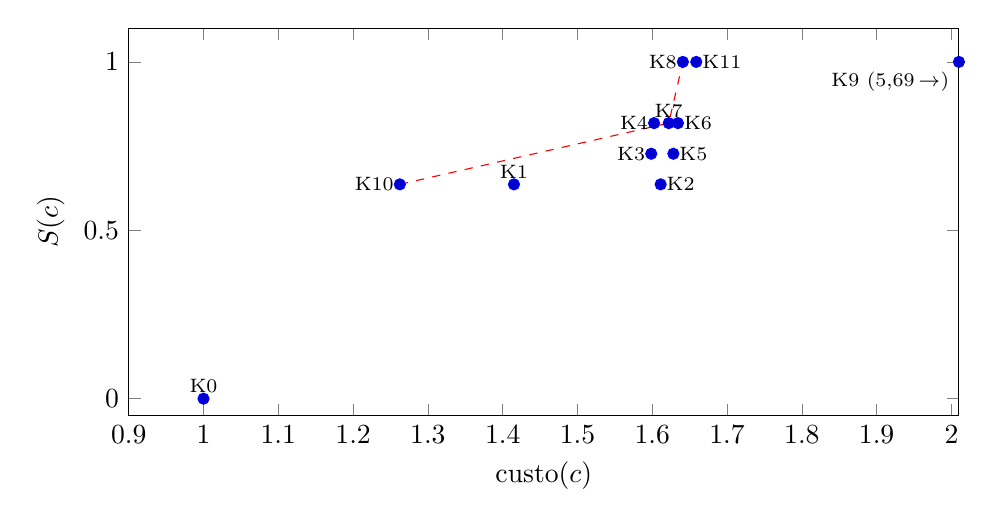
\begin{tikzpicture}
  \begin{axis}[width=\linewidth, height=6.5cm, xlabel={custo$(c)$},
      ylabel={$S(c)$}, ymin=-0.05, ymax=1.1, xmin=0.9, xmax=2.01,
      clip=false]
    \addplot+[only marks] coordinates {
      (1.0,0.0)
      (1.4151,0.6364)
      (1.6112,0.6364)
      (1.5986,0.7273)
      (1.6024,0.8182)
      (1.6282,0.7273)
      (1.6343,0.8182)
      (1.622,0.8182)
      (1.6409,1.0)
      (2.01,1.0)
      (1.2625,0.6364)
      (1.6588,1.0)
    };
    \addplot+[no marks, dashed] coordinates {
      (1.2625,0.6364)
      (1.622,0.8182)
      (1.6409,1.0)
    };
    \node[anchor=south, font=\scriptsize, inner sep=2pt] at (axis cs:1.0,0.0) {K0};
    \node[anchor=south, font=\scriptsize, inner sep=2pt] at (axis cs:1.4151,0.6364) {K1};
    \node[anchor=west, font=\scriptsize, inner sep=2pt] at (axis cs:1.6112,0.6364) {K2};
    \node[anchor=east, font=\scriptsize, inner sep=2pt] at (axis cs:1.5986,0.7273) {K3};
    \node[anchor=east, font=\scriptsize, inner sep=2pt] at (axis cs:1.6024,0.8182) {K4};
    \node[anchor=west, font=\scriptsize, inner sep=2pt] at (axis cs:1.6282,0.7273) {K5};
    \node[anchor=west, font=\scriptsize, inner sep=2pt] at (axis cs:1.6343,0.8182) {K6};
    \node[anchor=south, font=\scriptsize, inner sep=2pt] at (axis cs:1.622,0.8182) {K7};
    \node[anchor=east, font=\scriptsize, inner sep=2pt] at (axis cs:1.6409,1.0) {K8};
    \node[anchor=north east, font=\scriptsize] at (axis cs:2.01,1.0) {K9 (5,69\,$\rightarrow$)};
    \node[anchor=east, font=\scriptsize, inner sep=2pt] at (axis cs:1.2625,0.6364) {K10};
    \node[anchor=west, font=\scriptsize, inner sep=2pt] at (axis cs:1.6588,1.0) {K11};
  \end{axis}
\end{tikzpicture}
